\documentclass[pdf,sprung,slideColor,nocolorBG]{beamer}
%
%\documentclass[hyperref={pdfpagelabels=false}]{beamer}
\mode<presentation>

\newenvironment{colortheme}[1]{
\def\ProvidesPackageRCS $##1${\relax}
\renewcommand{\ProcessOptions}{\relax}
\makeatletter
\input beamercolortheme#1.sty
\makeatother
}{}

\let\Tiny=\tiny
\usetheme{ACCESS}
\usefonttheme{structurebold}
\setbeamerfont{structure}{series=\bfseries}
\setbeamertemplate{frametitle}[default][center]
\usepackage{svg}
\svgsetup{}
\usepackage[figurename={}]{caption}
%\usepackage[latin1]{inputenc}
%\usepackage{amsmath}   %needed for \begin{align}... \end{align} environment
\usepackage{amsfonts}
\usepackage{amssymb}
\usepackage{amscd}
\usepackage[all]{xy}
\usepackage{xcolor}
\usepackage{enumerate}
%
\newcommand{\slidecite}[1]{\tiny{(#1)}\normalsize{}}
\newcommand{\smallcite}[1]{\small{(#1)}\normalsize{}}
\newcommand{\tinycaptionof}[2]{\captionof{#1}{\tiny{#2}}}

\newcommand{\mb}[1]{\mathbb{#1}}
\newcommand{\mf}[1]{\mathbf{#1}}
\newcommand{\Emph}[1]{\emph{\textcolor{blue}{#1}}}

\newcommand{\abs}[1]{\left| #1 \right|}
\newcommand{\norm}[1]{\left\| #1 \right\|}
\newcommand{\To}{\rightarrow}

\newcommand{\Cay}[1]{\operatorname{Cay}\left(#1\right)}
\newcommand{\Clique}[1]{\omega\left(#1\right)}
\newcommand{\dual}[1]{\widetilde{#1}}
\newcommand{\support}[1]{\operatorname{supp}\left(#1\right)}
\newcommand{\weight}[1]{\operatorname{wt}\left(#1\right)}
\newcommand{\weightclass}[1]{\operatorname{wc}\left(#1\right)}

\newcommand{\G}{\mb{G}}
\newcommand{\R}{\mb{R}}
\newcommand{\Z}{\mb{Z}}

\newcommand{\slidebg}[1]{\usebackgroundtemplate{
\vbox to \paperheight{
\vspace{+5em}
\includegraphics[width=\paperwidth,keepaspectratio]{#1}}}}
\newcommand{\noslidebg}{\usebackgroundtemplate{}}

\newcommand{\sectionslide}[1]{%
\section{#1}
\slidebg{../graphics/ACCESS-NRI-template-section.jpg}
\begin{frame}
\vspace{+4em}
\centering
\hspace{+3em}\textbf{\huge{#1}\normalsize{}}
\end{frame}
\noslidebg
}

%\newtheorem{Definition}{Definition}
\newtheorem{Question}{Question}
\newtheorem{Conjecture}{Conjecture}

\title{Big data in combinatorics: is it feasible?}
\author{Paul Leopardi}

\date{For 46 ACC Brisbane 2024}

\institute{ACCESS-NRI, Australian National University.}
\titlegraphic{
%\includegraphics[angle=0,width=10mm]{../../common/beamer-anu-colourlogo.png}
%\includegraphics[angle=0,width=20mm]{../../common/carma_logo.jpg}
}

\begin{document}
\begin{colortheme}{access}
\slidebg{../graphics/ACCESS-NRI-template-title.jpg}
\frame{\titlepage}

\slidebg{../graphics/ACCESS-NRI-template-page.jpg}
\begin{frame}
\frametitle{Acknowledgements}
\begin{center}

SageMath, Bliss, Nauty.

~

Bureau of Meteorology.

~

Australian National University.

~

National Computational Infrastructure.

~

ACCESS-NRI, NCRIS.
\end{center}
\end{frame}

\begin{frame}
\frametitle{Overview}
%\begin{center}
\begin{itemize}
\item
How big is big data?

~

~

\item
Some mathematical datasets

~

~

\item
A modest proposal

\end{itemize}

%\end{center}
\end{frame}
\end{colortheme}
\sectionslide{How big is big data?}

\begin{colortheme}{access}
\begin{frame}
\frametitle{Big data is becoming cheaper}
%
Hard disk costs have declined from \$41 per Terabyte in 2013 to \Emph{\$11 per Terabyte} in 2023 in constant US dollars

\begin{figure}
\centering
\begin{minipage}{\textwidth}
  \centering
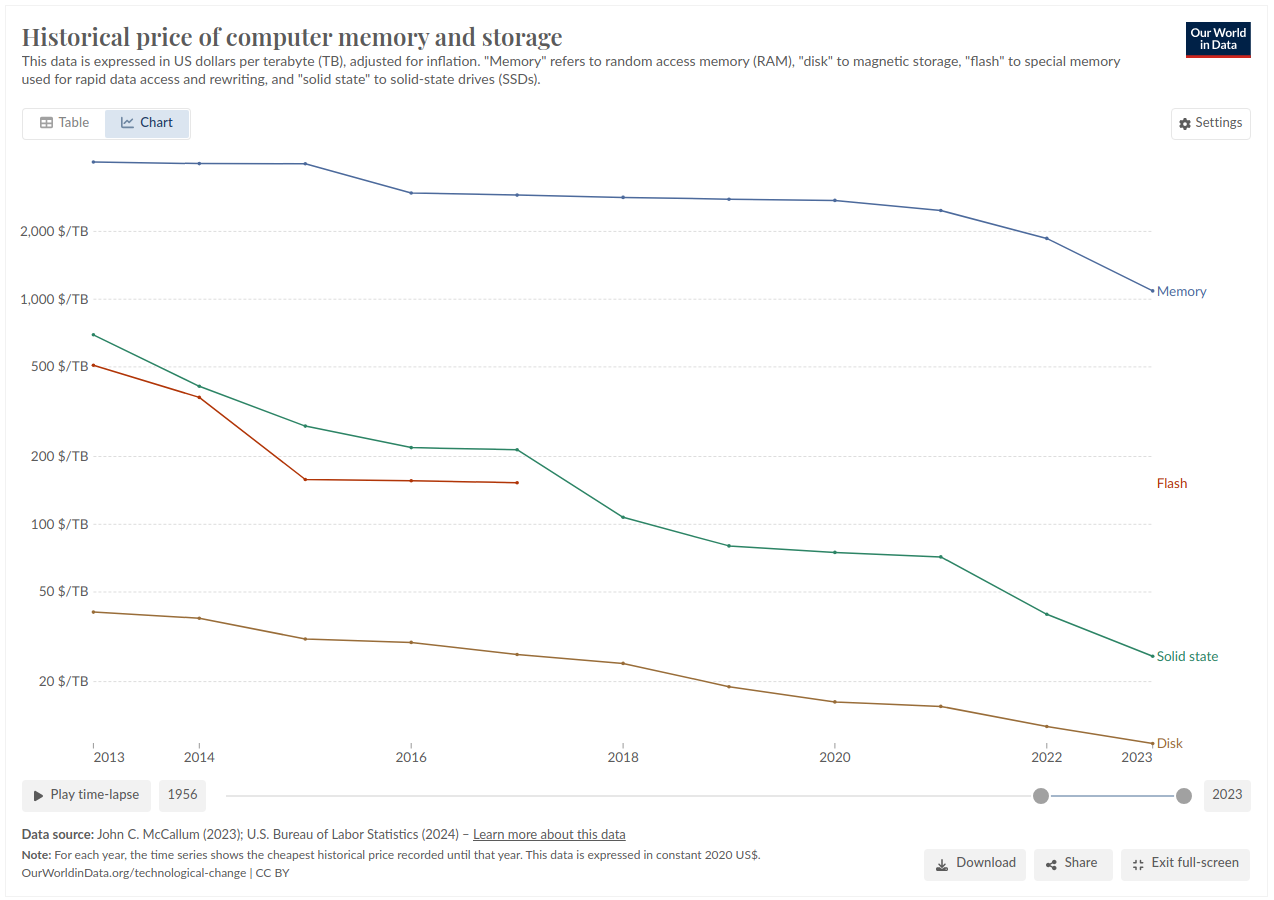
\includegraphics[width=.75\linewidth]{../graphics/Historical-price-of-storage.png}
  \vspace{-1em}
  \tinycaptionof{figure}{Historical price of computer memory and storage.\\
  Data source: John C. McCallum (2023); U.S. Bureau of Labor Statistics (2024)\\
  (https://ourworldindata.org/grapher/historical-cost-of-computer-memory-and-storage)}
  \label{fig:Historical-price}
\end{minipage}
\end{figure}
\end{frame}

\begin{frame}
\frametitle{The SKAO: 2 Petabytes per day}
%
The Square Kilometer Array Observatory will archive about

\Emph{2 Petabytes} of data \emph{per day}.
\begin{figure}
\centering
\begin{minipage}{\textwidth}
  \centering
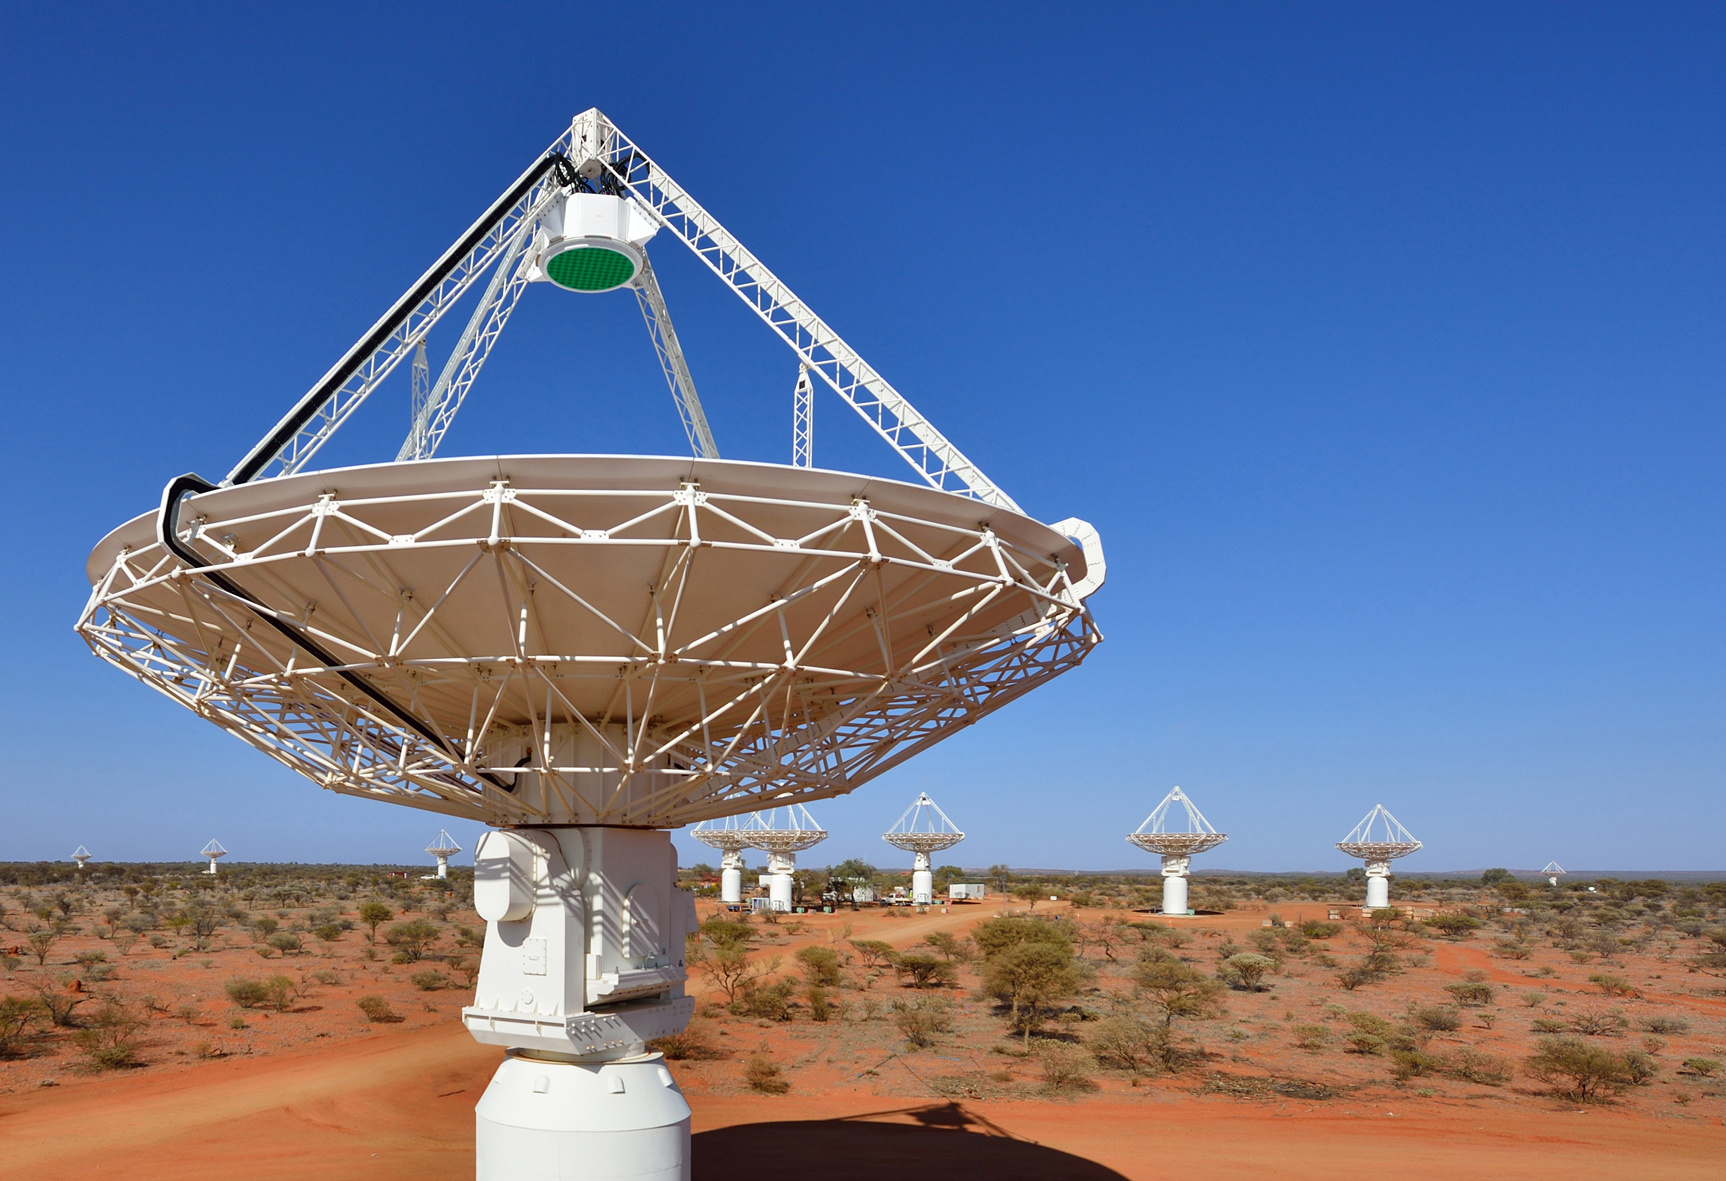
\includegraphics[width=.65\linewidth]{../graphics/CSIRO_ScienceImage_2161_Close_up_of_a_radio_astronomy_telescope_with_several_more_in_the_background.jpg}
  \tinycaptionof{figure}{CSIRO: Antennas of CSIRO's ASKAP telescope at the Murchison Radio-astronomy Observatory in Western Australia.}
  \label{fig:ASKAP}
\end{minipage}
\end{figure}
\vspace{-1em}
\slidecite{https://www.skao.int/en/explore/big-data 2024}
\end{frame}

\begin{frame}
\frametitle{ESGF: 16+ Petabytes of public databases}
%
The Earth System Grid Federation hosts climate datasets comprising more than \Emph{16 Petabytes} of data.
\begin{figure}
\centering
\begin{minipage}{\textwidth}
  \centering
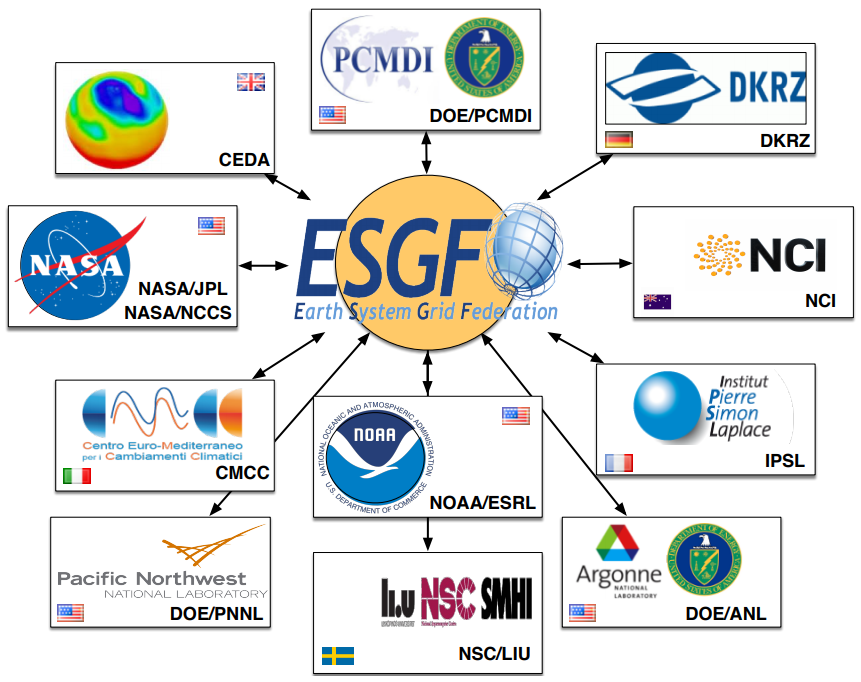
\includegraphics[width=.5\linewidth]{../graphics/ESGF-federation.png}
  \tinycaptionof{figure}{ESGF nodes 2018 (https://e3sm.org/wp-content/uploads/2018/03/ESGF-federation.png)}
  \label{fig:ESGF}
\end{minipage}
\end{figure}
\vspace{-1em}
\slidecite{Hoffmann et al. 2023}
\slidecite{https://www.climatemodeling.org/~forrest/presentations/Hoffman\_WCRP-OSC-ESGF\_20231023.pdf 2023}
\end{frame}

\begin{frame}
\frametitle{CERN ATLAS: 65 Terabyte public database}
%
In 2024 the ATLAS Experiment at CERN released approximately \Emph{65 Terabytes} of data collected in 2015 and 2016.
\begin{figure}
\centering
\begin{minipage}{\textwidth}
  \centering
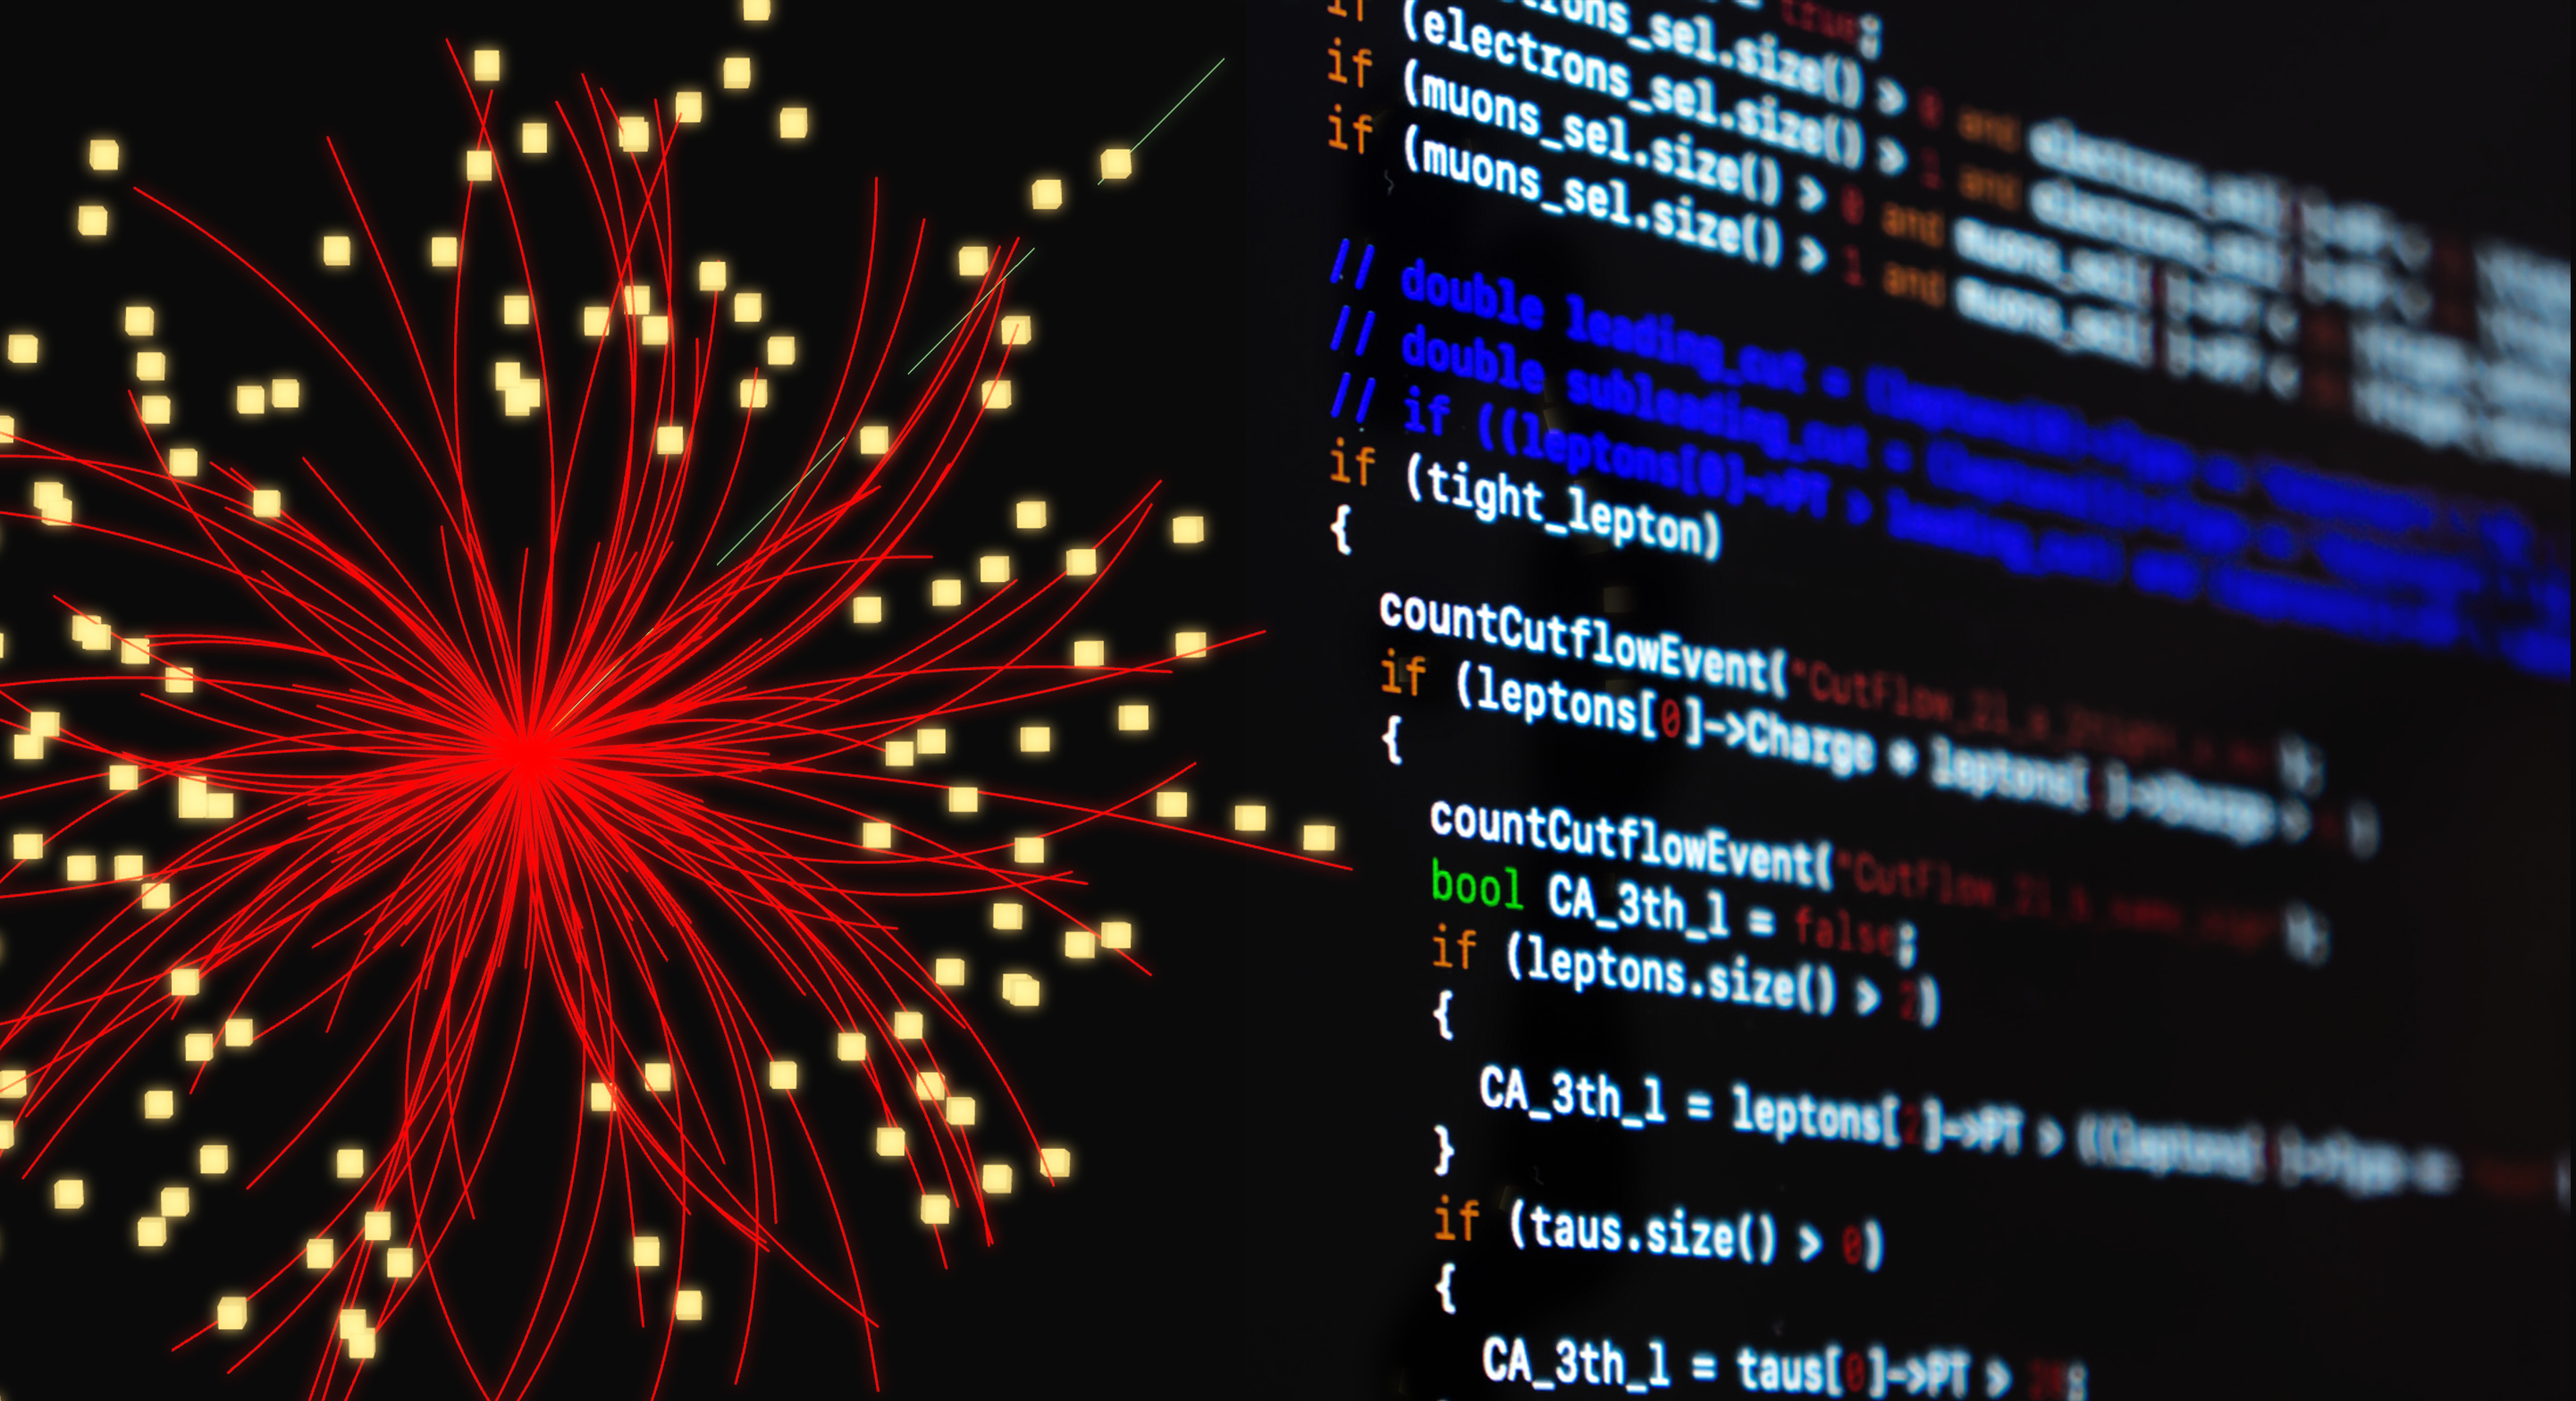
\includegraphics[width=.8\linewidth]{../graphics/ATLAS-open-data.jpg}
  \tinycaptionof{figure}{ATLAS open data 2024 (https://atlas.cern/sites/default/files/2024-07/ATLAS-open-data.jpg)}
  \label{fig:ATLAS}
\end{minipage}
\end{figure}
\vspace{-1em}
\slidecite{https://atlas.cern/Updates/News/Open-Data-Research 2024}
\end{frame}


\end{colortheme}

\sectionslide{Some mathematical datasets}
\slidebg{../graphics/ACCESS-NRI-template-page.jpg}

\begin{colortheme}{access}
\begin{frame}
\frametitle{The OpenDreamKit project}

The EU funded OpenDreamKit project (2015-2019) included a census of mathematical data sets,
and the development of prototypical semantic infrastructure for the FAIR sharing of such data sets.
This used the idea of ``Deep FAIR'': FAIR sharing at the level of mathematical objects.

\begin{figure}
\centering
\begin{minipage}{\textwidth}
  \centering
\includesvg[width=50mm]{../graphics/use-cases-lmfdb-mediator.svg}
  \tinycaptionof{figure}{Math in the Middle mediator, OpenDreamKit Project 2019}
  \label{fig:OpenDreamKit}
\end{minipage}
\end{figure}

\slidecite{OpenDreamKit Project 2015-2019; Ber\v{c}i\v{c}, Kohlhase and Rabe 2020}
\end{frame}

\begin{frame}
\frametitle{The L-functions and modular forms database LMFDB}
 \begin{itemize}
  \item
``The LMFDB is an extensive database of mathematical objects arising in Number Theory.''
  \item
Recently extended to include abstract groups.
  \item
About \Emph{2 Terabytes} in size.
 \end{itemize}

\begin{figure}
\centering
\begin{minipage}{\textwidth}
  \centering
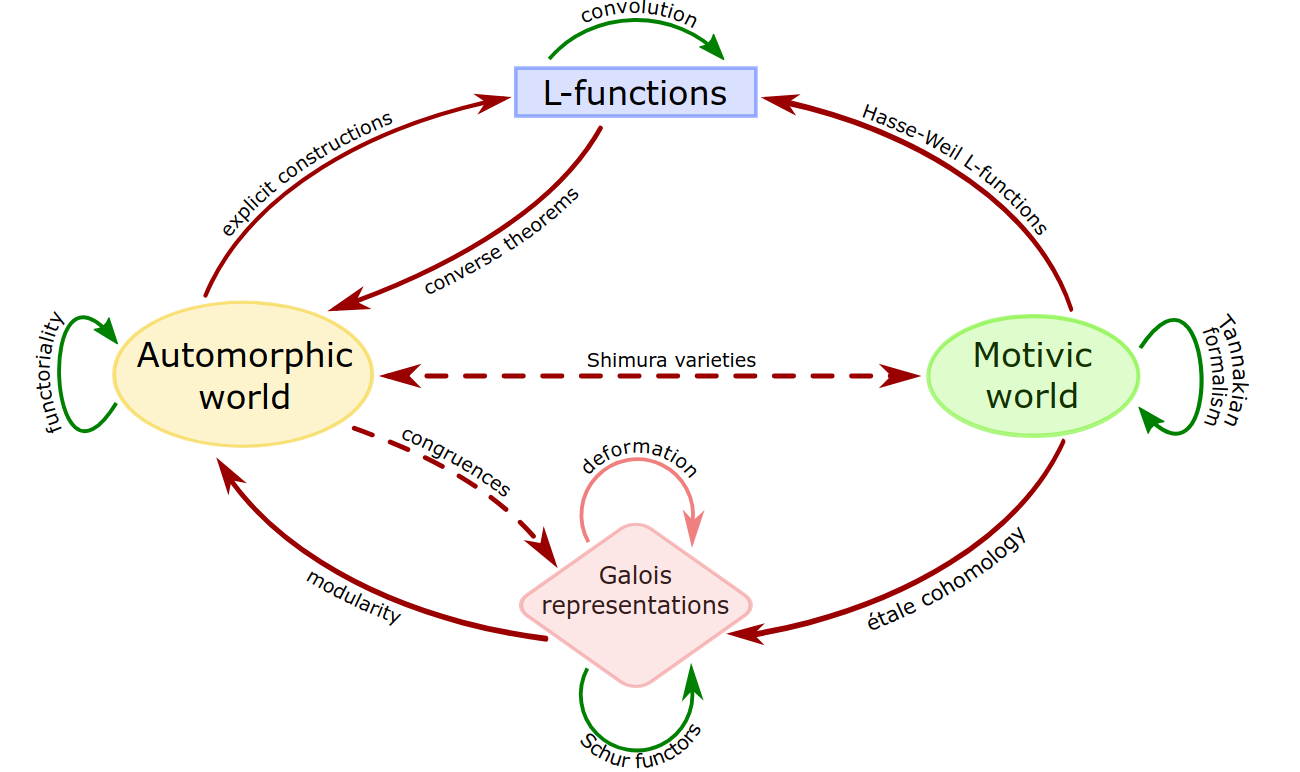
\includegraphics[width=.6\linewidth]{../graphics/LMFDB.png}
  \tinycaptionof{figure}{The LMFDB universe 2024}
  \label{fig:LMFDB}
\end{minipage}
\end{figure}
\vspace{-1em}
\slidecite{The LMFDB Collaboration 2024; Combes et al. 2024}
\end{frame}

\begin{frame}
\frametitle{House of Graphs: a database of interesting graphs}
 \begin{itemize}
  \item
``It is the aim of this House of Graphs project to find a workable definition of 'interesting' and provide a searchable database of graphs that conform to this definition.''
  \item
Grew from 1500 to \Emph{22 000 graphs} from 2012 to 2023.
  \item
Rebuilt as House of Graphs 2.0 in 2021-2022 to be more flexible and expandable.
  \item
Includes a directory of other graph databases.
  \item
Lean-HoG is a Lean 4 library with an interface to House of Graphs.
 \end{itemize}

 ~

\slidecite{Brinkmann et al. 2013; Coolsaet et al. 2023; Bauer, Ber\v{c}i\v{c} and Taslak 2024.}
\end{frame}

\begin{frame}
\frametitle{DiscreteZOO: A Fingerprint Database of Discrete Objects}
 \begin{itemize}
  \item
A data repository, a website and a SageMath Package for discrete combinatorial objects such as graphs with a high degree of symmetry.
  \item
As at 2020 it contains \Emph{212 269 graphs}.
 \end{itemize}

\begin{figure}
\centering
\begin{minipage}{\textwidth}
  \centering
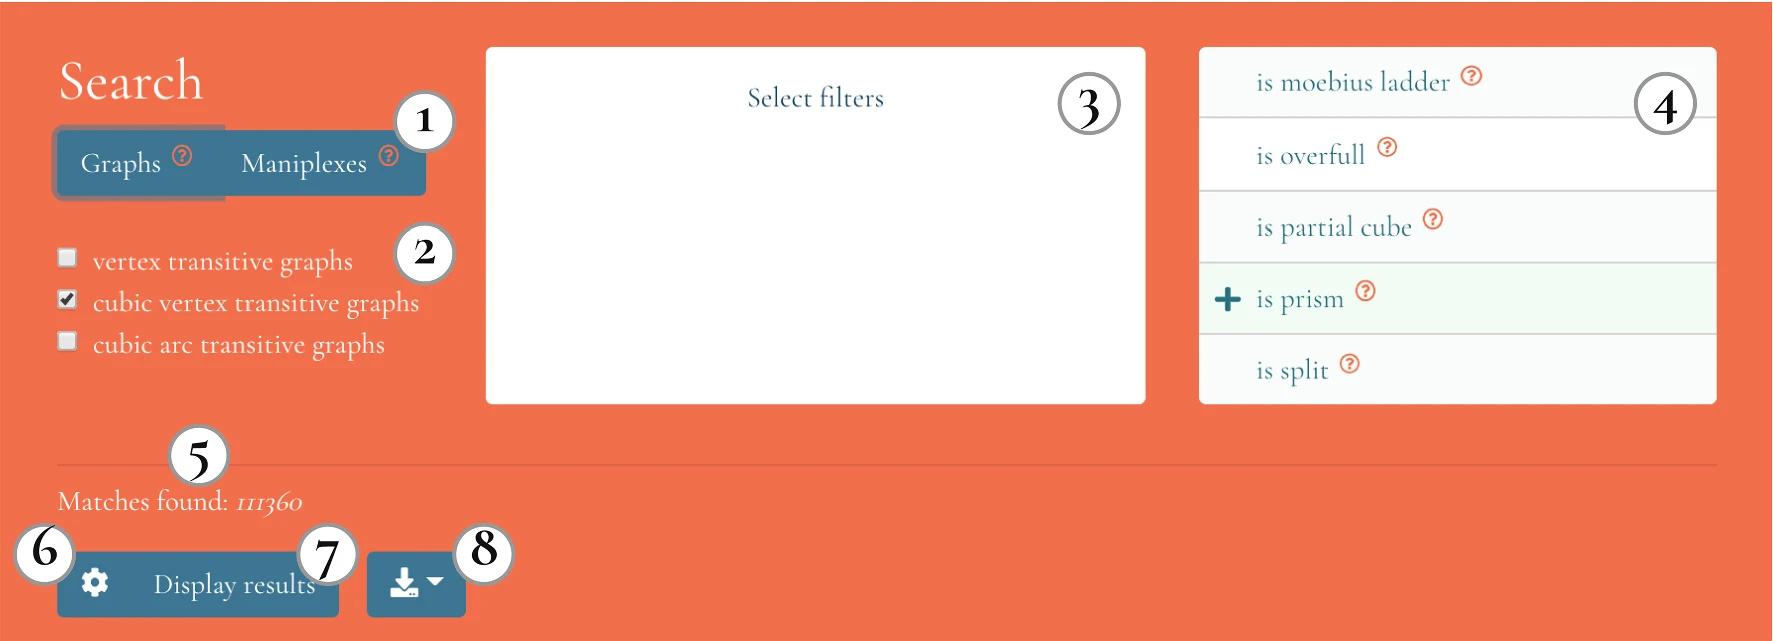
\includegraphics[width=.6\linewidth]{../graphics/DiscreteZoo-6.jpg}
  \tinycaptionof{figure}{DiscreteZoo search box 2020}
  \label{fig:DiscreteZOO}
\end{minipage}
\end{figure}
\vspace{-1em}
\slidecite{Ber\v{c}i\v{c} and Vidali 2020}
\end{frame}

\noslidebg
\begin{frame}
\frametitle{Datasets of strongly regular graphs}
\begin{itemize}
 \item
Spence's lists of strongly regular graphs on at most 64 vertices.
 \begin{itemize}
  \item
Exhaustive lists of non-isomorphic graphs for some tuples of feasible parameters.
  \item
Flat text files.
 \end{itemize}
 \item
Brouwer's database of parameters of strongly regular graphs.
 \item
Cohen and Pasechnik's Sage implementation of Brouwer's database, with constructions.
 \begin{itemize}
  \item
Example for each tuple of feasible parameters, if known.
  \item
Sage interface.
 \end{itemize}
 \item
Ihringer's lists of strongly regular graphs on at most 255 vertices.
 \begin{itemize}
  \item
\Emph{Over 34 GB} of lists containing more than \Emph{200 million graphs} generated by switchings.
  \item
Gzipped G6 files stored in Dropbox.
 \end{itemize}
\end{itemize}
\vspace{-0.5em}
\slidecite{Spence 1995-2006; Brouwer 2008-2017; Cohen and Pasechnik 2016-2017; Ihringer 2022}
\end{frame}


\slidebg{../graphics/ACCESS-NRI-template-page.jpg}
\begin{frame}
\frametitle{Use cases for datasets of strongly regular graphs}

\begin{enumerate}
 \item Test graph recognition algorithms.

 Many papers have been written on testing and extending the Weisfeiler-Lehman algorithm, using data sets of graphs.

 ~

 \item Obtain statistical distributions of properties of strongly regular graphs.

 ~

 \item Implement Roberson's classification of strongly regular graphs into four types according to clique number and chromatic number.
\end{enumerate}

~

\slidecite{Weisfeiler and Leman 1968; Babai 1980; Yang et al 2024; Cameron 2003; Roberson 2019}
\end{frame}

\end{colortheme}

\sectionslide{A modest proposal}

\begin{colortheme}{access}

\slidebg{../graphics/ACCESS-NRI-template-page.jpg}
\begin{frame}
\frametitle{Bent function Cayley graph data sets (1)}
Strongly regular graphs with parameters $(64, 28, 12, 12)$ and $(64, 36, 20, 20)$ as
Cayley graphs of bent functions in 6 dimensions.

Currently stored \textbf{on my desk at home}.

~
\begin{itemize}
  \item
Database of 11 strongly regular graphs from 4 extended translate (ET) classes.

~
  \item
SQLite database size is 780 KB.
 \end{itemize}

\end{frame}

\noslidebg
\begin{frame}
\frametitle{Bent function Cayley graph data sets (2)}
Strongly regular graphs with parameters $(256, 120, 56, 56)$ and $(256, 136, 72, 72)$ as
Cayley graphs of bent functions in 8 dimensions.
Currently stored \textbf{on my desk at home}.
\small{}
\begin{itemize}
\item
Bent functions in 8 dimensions up to degree 3.
 \begin{itemize}
  \item
Database of 55 strongly regular graphs from 9 ET classes.
  \item
SQLite database size is 65 MB.
 \end{itemize}
 \item
Bent functions from the 8 S-boxes of CAST-128.
 \begin{itemize}
  \item
Database of more than \Emph{32 million} ($32\,914\,496$) strongly regular graphs from 256 ET classes and their duals.
  \item
SQLite database size is \Emph{195 Gigabytes}.
 \end{itemize}
\item
About \Emph{2 billion} strongly regular graphs from
the 14 758 ET classes of partial spread bent functions in 8 dimensions and their duals.
 \begin{itemize}
  \item
Currently stored as SageMath sobj files.
  \item
\Emph{Over 6 Terabytes} total size.
 \end{itemize}
\end{itemize}

\end{frame}

\begin{frame}
\frametitle{Schema for Cayley graph databases}
\begin{figure}
\centering
\begin{minipage}{\textwidth}
  \centering
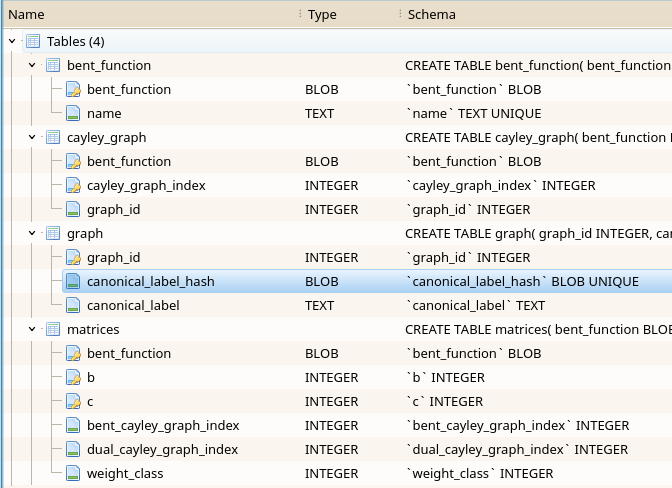
\includegraphics[width=.75\linewidth]{../graphics/Classification-schema-SQLite.png}
  \captionof{figure}{Database schema for SQLite version of the Cayley graph database.}
  \label{fig:Classification-schema-SQLite}
\end{minipage}%
\end{figure}
\end{frame}

\slidebg{../graphics/ACCESS-NRI-template-page.jpg}
\begin{frame}[fragile]
\frametitle{Bent function Cayley graph Sage code}

CoCalc: Public worksheets, Sage and Python source code

\begin{verbatim}
http://tinyurl.com/Boolean-Cayley-graphs
\end{verbatim}

~

GitHub: Sage and Python source code

\begin{verbatim}
https://github.com/penguian/Boolean-Cayley-graphs
\end{verbatim}

~

PyPI: Installable Python package


\begin{verbatim}
https://pypi.org/project/boolean-cayley-graphs/
\end{verbatim}

~

SourceForge: Documentation of Python modules

\begin{verbatim}
https://boolean-cayley-graphs.sourceforge.io/
\end{verbatim}

\end{frame}

\begin{frame}[fragile]
\frametitle{Possible next steps}

\begin{itemize}
 \item
\textbf{Find an academic collaborator}.

~

 \item
Revise and resubmit the paper, arXiv:1705.04507 [math.CO]


``Classifying bent functions by their Cayley graphs.''


~

 \item
Arrange for public hosting of the bent function Cayley graph databases.

~

 \item
Scale up to include the partial spread bent functions.
\end{itemize}

\end{frame}

\end{colortheme}

\section{}
\slidebg{../graphics/ACCESS-NRI-template-final.jpg}
\begin{frame}
\end{frame}

\end{document}
